\documentclass[11pt]{article}
\usepackage[italian]{babel}
\usepackage[utf8]{inputenc}
\usepackage{graphicx}
\usepackage{float}
\usepackage{amsmath}
\usepackage{amsfonts}
\usepackage{hyperref}
\usepackage{glossaries}
\makeglossaries
\newglossaryentry{domain}{
    name=domain,
    description={Si intendono, qui, le conoscenze relative ad un determinato ambito. Ad esempio, sviluppando un sistema per Trenitalia(\textit{qualcuno lo fa veramente? Non sono scritti da scimmiette?}), il dominio sarebbe quello della gestione dei treni. Il problema sta nel fatto che il programmatore non ha conoscenze al riguardo dei treni, e deve utilizzare quindi un linguaggio, implicazioni e conoscenze che non gli appartengono}
}
\newglossaryentry{volatility}{
    name=volatility,
    description={Con RV intendiamo modifiche ai requirements che avvengono durante lo sviluppo del progetto. \textit{(Il classico "Ah ma già che ci sei, mi aggiungi un ecommerce, una macchina del caffè, e la possibilità di accarezzare i clienti attraverso il computer? Maledetti)}}
}
\newglossaryentry{case}{
    name={CASE tool},
    description={Il CASE tool è un software che supporta la progettazione di sistemi software, ad esempio con UML}
}
\newglossaryentry{constraint}{
    name={constraint},
    description={un constraint è un limite che viene posto; restriction, limitation.}
}
\usepackage[normalem]{ulem}
\newcommand{\code}[1]{\texttt{#1}}
\newcommand{\numpy}{{\tt numpy}}    % tt font for numpy
\topmargin -.5in
\textheight 9in
\oddsidemargin -.25in
\evensidemargin -.25in
\textwidth 7in
\begin{document}

% ========== Edit your name here
\author{Simone Montali}
\title{Riassunti di Ingegneria del Software}

\maketitle

\medskip

\section{T1 - Software Development Process}
Anche la signora seduta all'angolo di via Cavour, sa che oggi più che mai i software sono parte di tutti i processi che fanno girare il mondo. L'Ingegneria del software è però molto di più che scrivere codice. Infatti, è piuttosto un concetto di risoluzione dei problemi del mondo reale, sfruttando software. I requirements sono sempre più stringenti: tempi brevi, sistemi complessi, molte funzionalità richieste. Un buon software deve avere ottime \textbf{maintainability, dependability, efficiency, acceptability}. Problemi e soluzioni sono complessi, ma il software offre estrema flessibilità. Esso è un sistema discreto. Alcuni problemi tipici possono essere le scadenze, i budget, le performance, la manutenzione. Le sfide principali sono rappresentate da \textbf{eterogeneità, delivery, trust.} L'attività di problem solving è composta da due fasi: l'analisi e la sintesi. 
\subsection{Quindi? Cos'è l'ingegneria del software?}
Siamo giunti al nocciolo della questione: \textbf{di cosa stiamo parlando?} L'ingegneria del software è un insieme di \textbf{tecniche, metodologie, strumenti} che aiutano nella produzione di software di alta qualità dati un budget, una scadenza, e delle modifiche continue. La sfida principale è quindi quella di avere a che fare con complessità elevate. 
Siamo di fronte anche a un aumento delle responsabilità: un ingegnere del software non deve solo scrivere codice, ma piuttosto lavorare con competenze e confidenzialità, applicando un'etica.
\subsubsection{Processo del software}
In seguito ad una rappresentazione astratta, si procede con un set di attività strutturato: specifica dei \textbf{requirements}, \textbf{design}, \textbf{implementazione}, \textbf{validazione},\textbf{evoluzione}. 
\subsection{Modelli di sviluppo del software}
Distinguiamo tra \textbf{plan-driven} e \textbf{agile} development. Nel primo, prima si pianificano i requirement, e solo in seguito si sviluppa il software. Nel secondo si sviluppa il software un pezzo alla volta, a stretto contatto col cliente. 
\subsubsection{Modello a cascata}
In questo modello, \textbf{plan-driven}, le specifiche e lo sviluppo sono separati. I pro sono, ad esempio, un'ottima documentazione e manutenzione semplice. D'altro canto, però, le specifiche vengono \textit{"congelate"} dopo la prima fase, il cliente viene poco coinvolto, ed i tempi sono più lunghi. 
\begin{figure}[H]
    \centering
    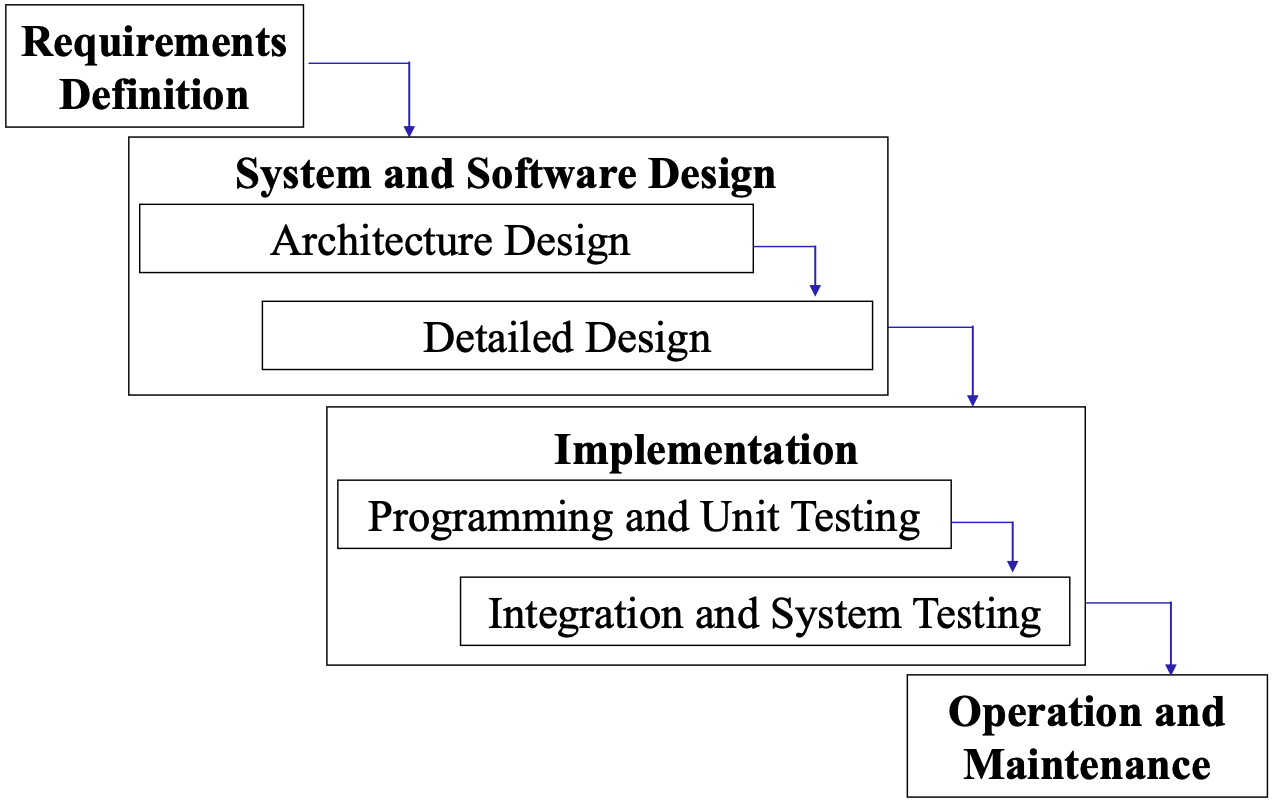
\includegraphics[width=\linewidth]{res/teoria/WaterfallModel.png}
    \caption{Waterfall Model}
\end{figure}
\subsubsection{Modello a spirale}
Nel modello a spirale, abbiamo diverse fasi che si susseguono a spirale; il \textit{risk handling} viene gestito tramite prototipazione, che permette di testare i prodotti contro i requirements. Alcuni pro possono essere l'elevata prevenzione dei rischi, la completezza della documentazione, la flessibilità. È, però, un modello costoso, riservato ad esperti ed a progetti costosi e richiedenti molta sicurezza. La spirale può allargarsi all'infinito. Il \textbf{prototipo} è un'implementazione limitata del sistema, rappresentando solo alcuni aspetti. È utilizzato in varie fasi dello sviluppo. Porta però vari vantaggi, come un'elevata usabilità, un buon design, una grande facilità di manutenzione, ed un ridotto costo di sviluppo. 
\begin{figure}[H]
    \centering
    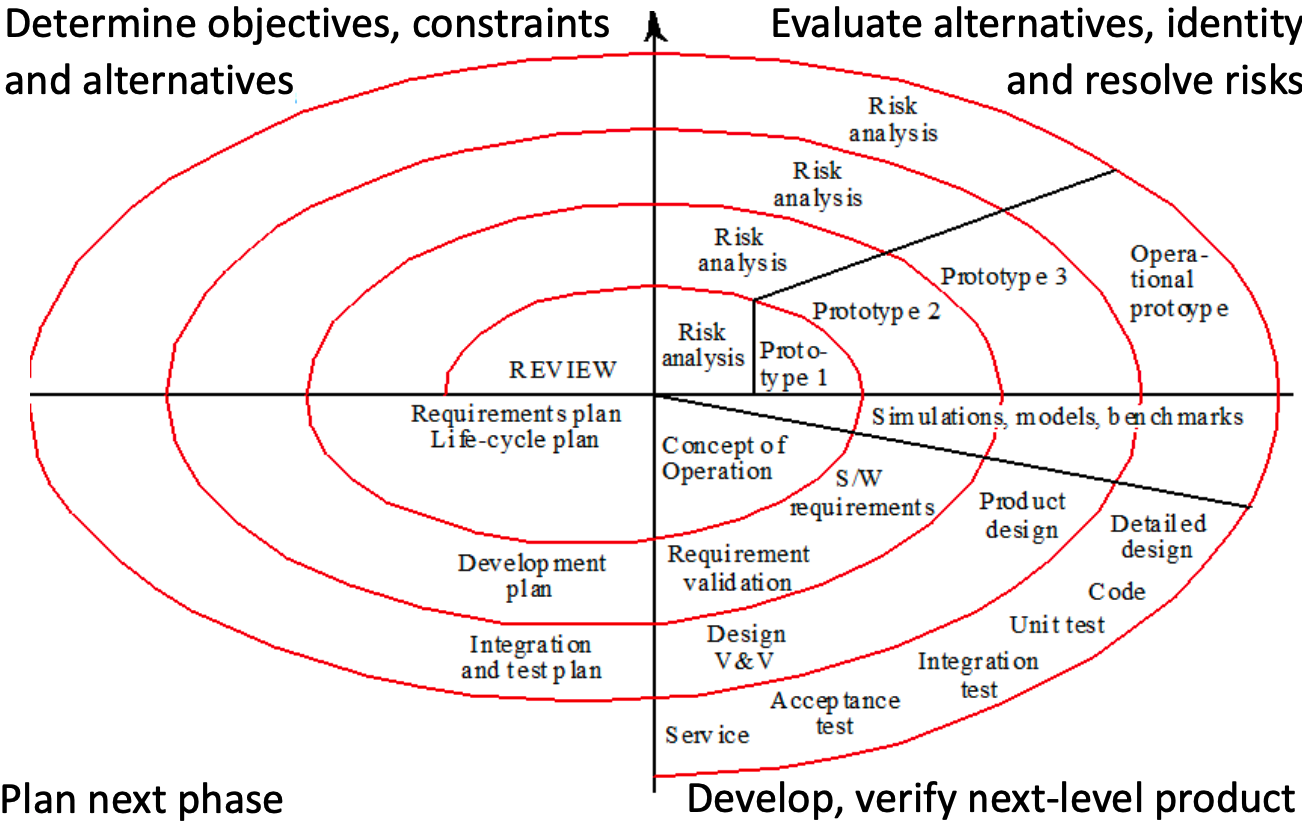
\includegraphics[width=\linewidth]{res/teoria/SpiralModel.png}
    \caption{Spiral Model}
\end{figure}
\subsubsection{Incremental development}
L'incremental development consiste in una prima fase di raccolta dei requirement, da cui nasce la versione iniziale, una fase di design, ed una fase di implementazione, che produce la versione finale. Alcuni pro possono essere la naturale presenza di prototipi ad ogni aggiunta di feature, un basso rischio di fallimento progettuale, una quantità di testing variabile in base alla priorità. Alcuni contro: bassa \textit{process visibility}, sistemi mal strutturati, skill speciali necessarie. Esso è adatto per progetti piccoli, o parti di progetti grandi. 
\begin{figure}[H]
    \centering
    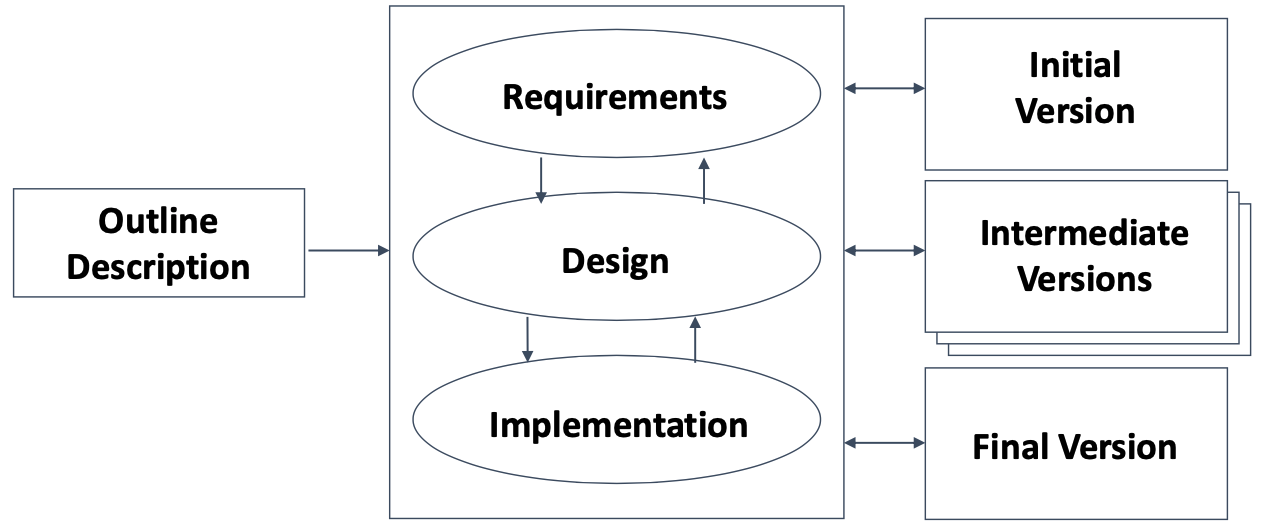
\includegraphics[width=\linewidth]{res/teoria/IncrementalDevelopment.png}
    \caption{Incremental Development}
\end{figure}
\subsubsection{Test driven development}
Qui, i test vengono scritti prima dell'implementazione, rendendo note le difficoltà da subito. Rende il debug più semplice. Si aggiunge un test, si prova il codice vecchio con il test nuovo, si aggiunge la feature e si verifica che il test sia ancora positivo. 
\subsubsection{Agile development}
\textit{"Tutti fanno Agile, nessuno fa Agile."}L'agile è basato sulla \textbf{continuous delivery}, con dei requirements in continuo cambiamento. Il cliente è direttamente coinvolto, aggiungendo requirements man mano che il progetto va avanti. È una metodologia semplice nella quale il team si auto organizza, ma ha svariati rischi, come la mancanza di planning, la necessità di team esperti, la documentazione scarna o spesso errata. 
\subsubsection{Extreme Programming}
\textit{Suona più badass di quanto sia realmente. /s} L'XP è utilizzato in situazioni in cui i requirements variano velocemente, i team sono ridotti e "affiatati"(spesso si ricorre al \textbf{pair programming}). È un tipo di programmazione agile, basato su design semplice, release minori, refactoring continuo, alta semplicità. 
\begin{figure}[H]
    \centering
    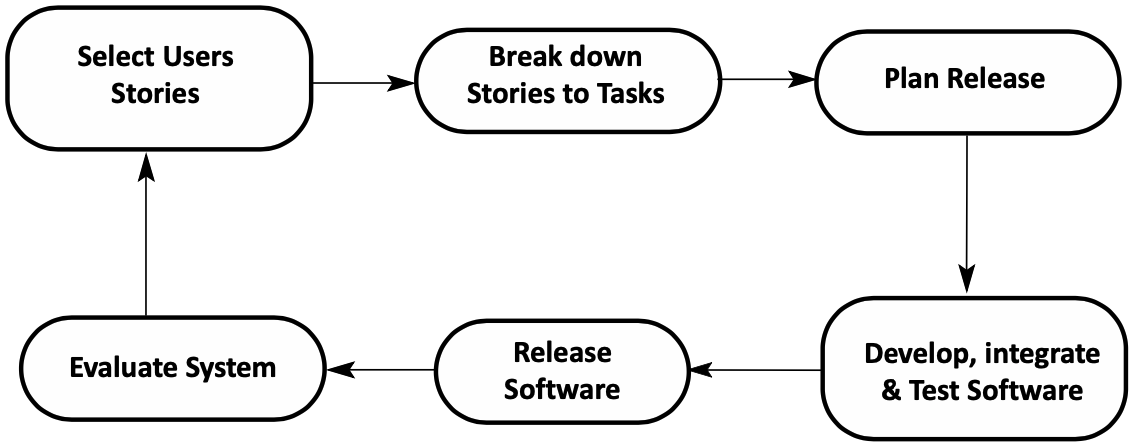
\includegraphics[width=\linewidth]{res/teoria/ExtremeProgramming.png}
    \caption{Extreme Programming}
\end{figure}
\subsection{Reusable software}
È spesso comodo lavorare per \textbf{microservizi} atomici, in modo da poterli riutilizzare. Parliamo, ad esempio, di API. Questo riduce i costi e i tempi di sviluppo, al costo di leggeri sacrifici sul lato dei requirements, e un mancato controllo sull'evoluzione del software $\rightarrow$ funzionalità che variano il loro comportamento. \textit{Parlo a lei, signor React (ah, già, Mark), che cambia tutto ad ogni versione.} 

\section{T2 - Coding, Debugging, Testing} 
Un buono stile di coding è fondamentale perché i programmi vengono scritti una volta, ma letti molte. Alcuni aspetti importanti sono il layout, i nomi, i commenti. 
\subsection{Legge di Ambler per gli standard}
Più uno standard è utilizzato, più è facile comunicare tra membri del team. Si possono inventare standard quando necessario, ma attenzione a non perdere tempo in qualcosa che non verrà riutilizzato. 
Tutti i linguaggi hanno standard reperibili. \textit{Consiglio per la vita: quando vi servono, esistono http://google.github.io/styleguide/gli standard di Google, gente più affidabile di me.} È consigliabile avere standard aziendali. Uno standard consiste di nomenclature, formattazione, formato e contenuto dei commenti. È necessario documentare tutte le volte in cui si infrangono gli standard. \textit{(È davvero necessario infrangerlo?)}
\subsection{Coding practices}
Alcune pratiche sono rappresentate da:
\begin{itemize}
    \item \textbf{indentazione}, che oltre ad essere importante per la leggibilità, a volte fa parte delle regole di compilazione. \textit{e.g. Python.}
    \item \textbf{whitespaces}, migliorano la leggibilità. \textit{Però, non fate le bestie di satana mettendo uno spazio dopo l'apertura della parentesi. Non fatelo. }
    \item \textbf{Naming, commenting}, rendono la comprensione del codice molto più facile.
\end{itemize}
I commenti sono uno strumento fondamentale da tenere sempre vicino al codice. Non pensiate però di essere autorizzati a scrivere \textit{spaghetti code}, se commentato. Refactorate. Fondamentale è spiegare i compiti di classi, funzioni, variabili o blocchi di codice complessi. \textit{In generale, se avreste bisogno di spiegarlo a Guido Soncini, commentatelo}. Utilizzare uno standard permette ai vostri colleghi di non dover riscrivere il vostro codice perché non gli piace. Rendete più semplice agiungere funzioni, o creare la documentazione. È, insomma, tempo ben speso. 
\subsection{Dealing with errors}
Distinguiamo tra prima, durante e dopo: \textbf{prevention, detection, recovery}. Alcune fonti di errori possono essere un design errato, una mancanza di isolazione, o typos. Per esempio, errori di "confini" negli array, errori di \textit{off-by-one}, errori di input errati. Per debuggare, bisogna riconoscere l'esistenza di un bug, isolarne la fonte, identificarne la causa, trovare un fix, applicarlo, e \textbf{testarlo}. \textit{Lo scrivo in grassetto perché mi capita spesso di romperepiù di quello che metto a posto.} 
Riconoscere un bug spesso è complicato, soprattutto quando accade solo in determinate situazioni, o se il software è difficile da testare. Per trovare i bug, potete usare dei print statement, molto veloci da usare ma spesso incompleti e poco pratici. Per questo, esistono gli strumenti di debug, che permettono di bloccare il codice in determinati punti, analizzare le variabili, \textit{e bestemmiare con calma.} Spesso gli errori sono dovuti al design piuttosto che all'implementazione. 
\subsection{Testing}
Il testing permette di scovare errori e bug, ma non la loro assenza. È purtroppo impossibile testare ogni caso. Il tester deve conoscere il sistema e le tecniche di testing. \textbf{Il tester non dovrebbe essere il programmatore.} Spesso il programmatore ha in mente il modo corretto di far funzionare il programma, e quindi difficilmente trova casi in cui il suddetto si rompe. 
\subsubsection{Unit testing}
Lo unit testing permette di testare singole unità di codice, trovando falle negli algoritmi, i dati, la sintassi. Un set di test cases viene creato e poi utilizzato. 
\subsubsection{Integration testing}
L'integration testing prova un gruppo di sottosistemi, o anche l'intero software. Viene eseguito dai programmatori, il goal è testare le interfacce oltre ai sottosistemi. 
L'intero sistema è visto come un insieme di sottosistemi, l'obiettivo è quello di testare tutte le interfacce e l'interazione tra sottosistemi. La strategia determina il modo in cui i sottosistemi vengono testati. Molte falle sono date da problemi nell'interazione tra sottosistemi. Le falle non intercettate in questa fase diventeranno molto più costose. 
\subsubsection{System Testing}
Il system testing testa l'intero sistema, per verificare che rispetti i requirements funzionali e non, oltre alle prestazioni. 
\subsubsection{Functional Testing}
Questo tipo di testing viene svolto per verificare la funzionalità del sistema. I test cases vengono ideati a partire dai requirement del progetto, ed il sistema è trattato come una black box. 
\subsubsection{Performance Testing}
Questo tipo di testing tenta di provare il sistema in situazioni estreme, come alti carichi, input errati, grandi volumi di dati. Alcuni esempi sono stress testing, security testing, volume testing, recovery testing.
\subsubsection{Acceptance Testing}
Questo tipo di testing prova che il sistema sia effettivamente pronto per la fase di production. I test vengono scelti ed effettuati dal cliente. Questi sono i famosi \textbf{alpha e beta tests.} Nel primo, il software è ancora nell'environment di sviluppo. Nella beta, l'environment è quello del cliente e l'utilizzo effettuato è realistico. 
\section{T3 - System Modeling and UML}
Il system modeling fornisce rappresentazioni astratte a problemi reali, tramite notazione grafica. Un modello funzionale dovrebbe introdurre i componenti essenziali, utilizzare una notazione \textit{consistente}, ed utilizzare tool al supporto della creazione. Il modello esprime quindi la realtà, adattata a dei modelli standard. Il system modeling deve essere \textbf{predictive}, in quanto deve essere svolto prima del development. Dev'essere \textbf{extracted} da un sistema esistente, tramite analisi delle proprietà del software. Deve essere \textbf{prescriptive}, ossia definire un set di regole e limiti per l'evoluzione del software. 
\subsection{UML}
Unified Modeling Language nasce per unire diversi standard/linguaggi di modellazione, con diagrammi multipli e interoperabilità. UML è \textbf{semplice, espressivo, utile, consistent, estensibile}. Alcuni esempi di views sono:
\begin{itemize}
    \item Use Case view
    \item Structural view
    \item Behavioral view
    \item Implementation view
    \item Environment view
\end{itemize}
\begin{figure}[H]
    \centering
    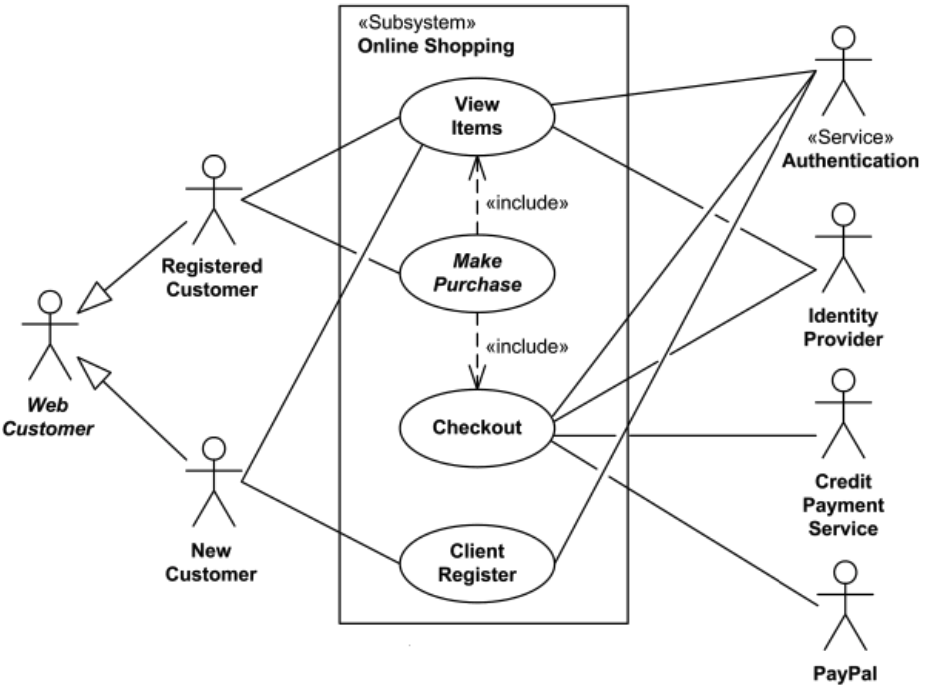
\includegraphics[width=0.6\linewidth]{res/teoria/UseCase.png}
    \caption{Use case diagram}
\end{figure}
\begin{figure}[H]
    \centering
    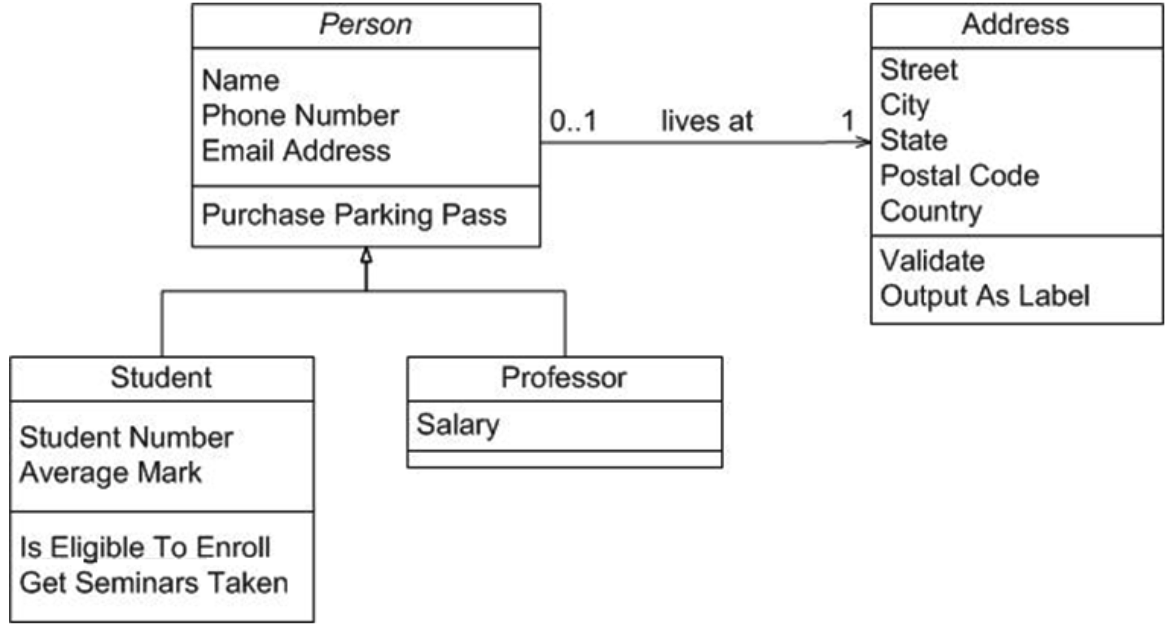
\includegraphics[width=0.6\linewidth]{res/teoria/ClassDiagram.png}
    \caption{Class diagram}
\end{figure}
\section{T4 - Requirements Engineering}
Gli scopi del requirements engineering sono \textbf{identificare} i servizi necessari ed i constraint, \textbf{definire} offerta e contratto, \textbf{ottenere} tutte le informazioni necessarie al design. I desiderata sono:
\begin{itemize}
    \item \textbf{Validi}, esprimendo le reali necessità
    \item \textbf{Non ambigui}, leggibili in un solo modo 
    \item \textbf{Completi}
    \item \textbf{Comprensibili} da tutte le persone coinvolte 
    \item \textbf{Consistent}, non possono contraddirsi 
    \item \textbf{Prioritizzati}, a volte bisogna scegliere
    \item \textbf{Verificabili}, con test 
    \item \textbf{Modificabili} senza difficoltà
    \item \textbf{Traceable}, la loro origine è chiara
\end{itemize}
\subsection{Some requirements classifications}
\subsubsection{Functional requirements (System Feature)}
Descrivono funzionalità di sistema o di servizi, come l'input di dati, operazioni svolte, workflow, dati in output, autorizzazioni. Ad esempio, in una biblioteca, un functional requirement può essere la ricerca di libri da parte di un socio.
\subsubsection{Non-functional requirements (System Feature)}
Descrivono \glspl{constraint} di parti del sistema e del suo sviluppo. Specificano criteri per giudicare l'operato del sistema. Con l'esempio di prima, i libri devono avere un codice che rispetti lo standard ISBN, e il sistema non deve rilasciare informazioni sensibili sui soci a determinati autorizzati. 
Alcune metriche per questi requirements possono essere velocità, dimensione, facilità d'uso, affidabilità, robustezza, portabilità.
\subsubsection{Domain requirements (System Feature)}
I \gls{domain} requirements derivano dal dominio dell'applicazione, ossia l'ambito in cui si lavora. 
\subsubsection{Volatile Requirements (Static/Dynamic Nature)}
I \textbf{mutable requirements} sono requirements destinati a cambiare, come normative o tasse. Gli \textbf{emergent requirements} cambiano quando il cliente capisce di più sul sistema. I \textbf{consequential requirements} emergono con l'informatizzazione di un sistema che non lo era. I \textbf{compatibility requirements} emergono dal doversi interfacciare con altri sistemi appartenenti all'organizzazione. 
\subsection{Rischi}
Alcuni rischi nella scrittura dei requirements possono essere:
\begin{itemize}
    \item Imprecisioni
    \item Conflitti tra più requirements
\end{itemize}
\subsection{Documento di specifica dei requirements}
Il \textbf{documento di specifica dei requirements} specifica i requirement di sistema, includendone una definizione e una specifica. È detto \textbf{System Specification} se include direttive su hardware e software, \textbf{Software Requirements Specification} (SRS) se include il solo software. Dovrebbe seguire lo standard IEEE 830. Un SRS deve avere un'\textbf{introduzione}, una \textbf{descrizione generale} ed infine \textbf{le feature e i requirement.} Dovrebbe avere un formato stratificato, notazioni grafiche e termini consistenti, acronimi chiari, indice, glossario, ed uno stile non ambiguo. A tal proposito, il linguaggio naturale spesso nasconde delle insidie: mancanza di chiarezza, ambiguità, troppa flessibilità... Bisogna quindi inventare uno standard di utilizzo del linguaggio naturale, con sintassi fissa, termini chiari. Alcune keyword sono: \textbf{shall, should, can, must, may, will, might, expected to, could.} Alcune alternative al linguaggio naturale possono essere un linguaggio naturale strutturato, linguaggi di descrizione del design, notazioni grafiche, notazioni formali. I rischi del processo di specifica sono una mancanza di comprensione, requirements che cambiano rapidamente, impreicisione nella stesura del documento, difficoltà nel conciliare conflitti. 

\section{T5 - Requirement engineering and UML}
\subsection{Use case diagram}
Nello use case diagram includiamo tutti i casi d'uso del sistema, da parte di diversi \textbf{attori}, rappresentanti utenti, ma anche servizi o sistemi. Il \textbf{system boundary} divide l'esterno e l'interno del sistema, gli use case dagli attori. Un attore può generalizzare un altro attore. Idem per gli use case. Uno use case può contenere la funzionalità di un altro use case. Uno use case può essere usato per estendere il comportamento di un altro use case, anche con condizioni. Opzionalmente, possiamo includere le molteplicità delle relazioni. 
\subsection{Class diagram}
Una classe è rappresentata da un rettangolo che mostra il nome della classe, e opzionalmente il nome degli attributi e delle operazioni. Il nome della classe, gli attributi e le operazioni sono separati in compartimenti. Il simbolo che precede attributi e operazioni ne indica la visibilità: $+$ se pubblico, $-$ se privato, $\#$ se protetto, $~$ se package. Un'\textbf{interfaccia} è una specifica di comportamento che deve essere implementato o, più semplicemente, un \textbf{contract.} Un \textbf{template} definisce un pattern i cui parametri rappresentano tipi, e può essere applicato a classi, packages, operazioni. 
\subsubsection{Associazione}
Un'associazione è una relazione tra elementi, che implica che uno dei due sia una variabile dell'altro. Essa è rappresentata da un connettore che può includere ruoli, cardinalità, direzione e \glspl{constraint}. Per più elementi, si può usare un \textbf{diamond}. 
\begin{figure}[H]
    \centering
    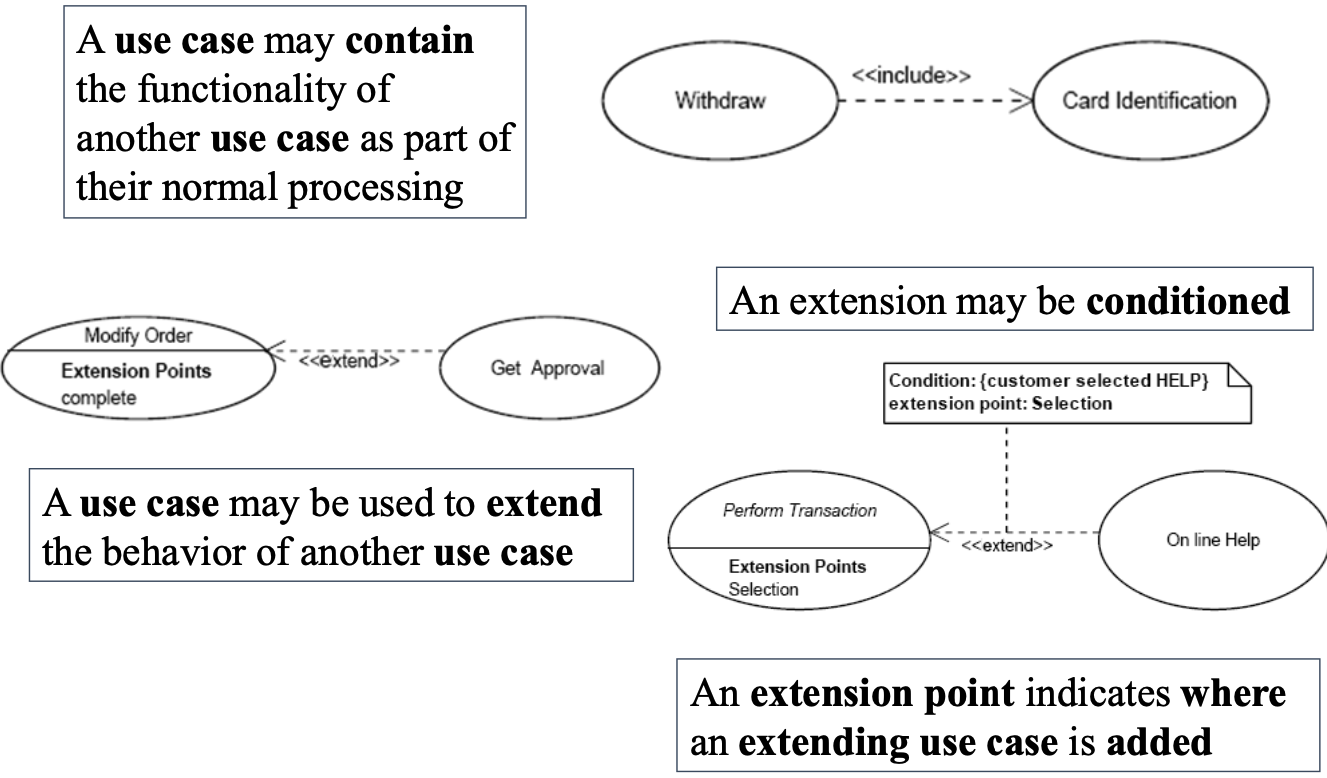
\includegraphics[width=0.6\linewidth]{res/teoria/Extension.png}
    \caption{Extension}
\end{figure}
\subsubsection{Generalization e nesting}
La generalizzazione indica \textbf{ereditarietà}, disegnata come una freccia che parte dal figlio e arriva al padre. Il connettore di nesting indica che una classe è nested nella classe dove arriva l'operatore. Con ciò, intendiamo che essa è definita all'interno del target. 
\begin{figure}[H]
    \centering
    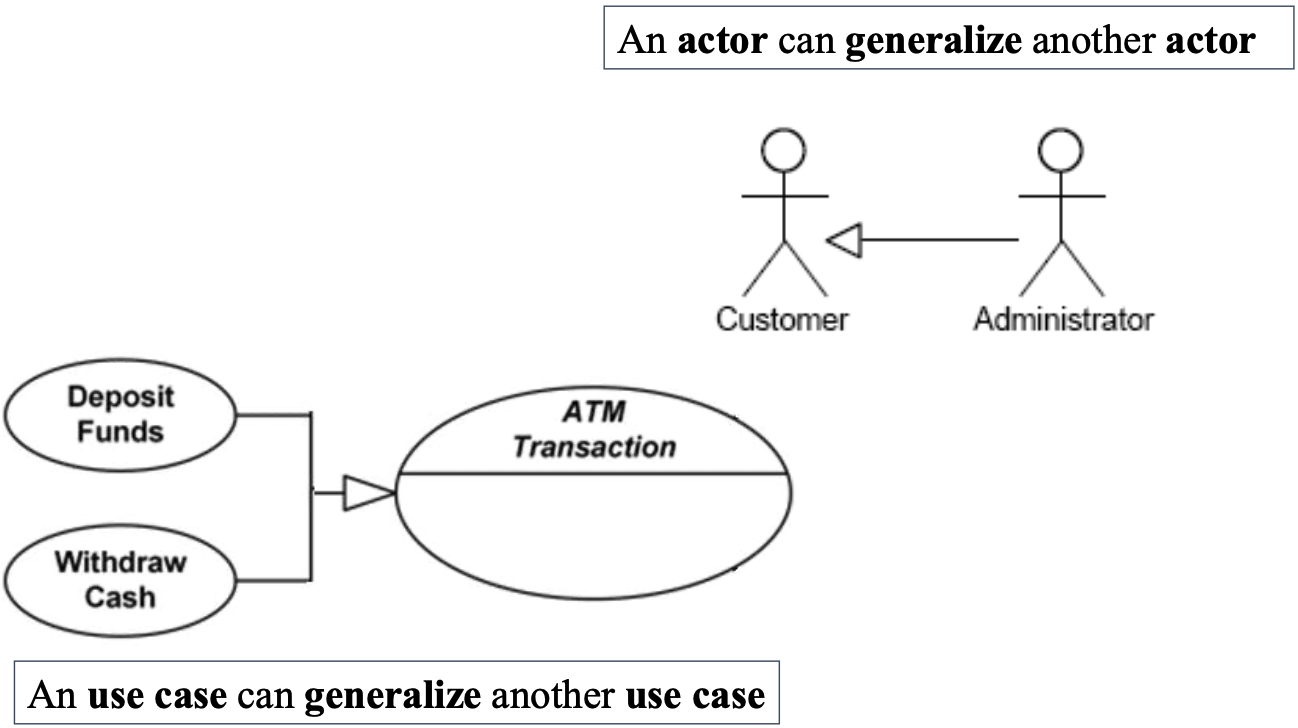
\includegraphics[width=0.6\linewidth]{res/teoria/Generalization.png}
    \caption{Generalization}
\end{figure}
\subsubsection{Dipendenza e realizzazione}
La \textbf{dipendenza} è una forma debole di relazione, e mostra un'interazione tra un client ed un supplier. La \textbf{realizzazione} è una relazione tra una specifica e la sua implementazione. 
\subsubsection{Aggregazione e composizione}
L'aggregazione rappresenta elementi composti da elementi minori. È indicata da un diamante bianco che punta verso il contenitore. I componenti possono essere condivisi da più contenitori. La composizione è rappresentata da un diamante nero. Una classe di associazione rappresenta invece un'associazione più complessa, che ha operazioni e attributi.
\begin{figure}[H]
    \centering
    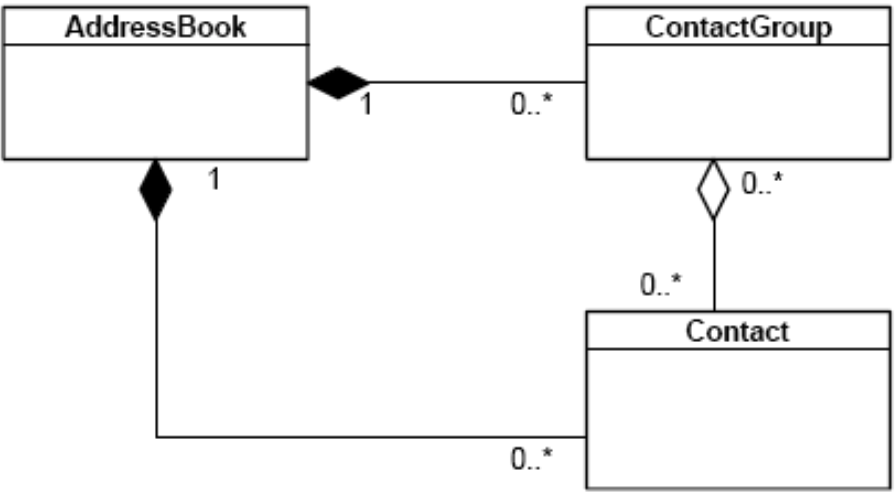
\includegraphics[width=0.6\linewidth]{res/teoria/AggrComposition.png}
    \caption{Aggregazione e composizione}
\end{figure}
\subsection{Sequence diagram} 
Il sequence diagram indica, su una \textit{lifeline (aka timeline)} verticale, l'interazione tra le classi. Se il nome della lifeline è \textit{self}, la suddetta rappresenta il classifier a cui appartiene il diagramma. Una \textbf{lifeline} rappresenta un \textit{partecipante} del sequence diagram. Possiamo avere diversi tipi di messaggi tra lifeline: sincroni, asincroni, risposte, persi, trovati, self (ricorsività). Per rappresentare logica procedurale come if, cicli, thread, usiamo i \textbf{fragment}. 
\begin{figure}[H]
    \centering
    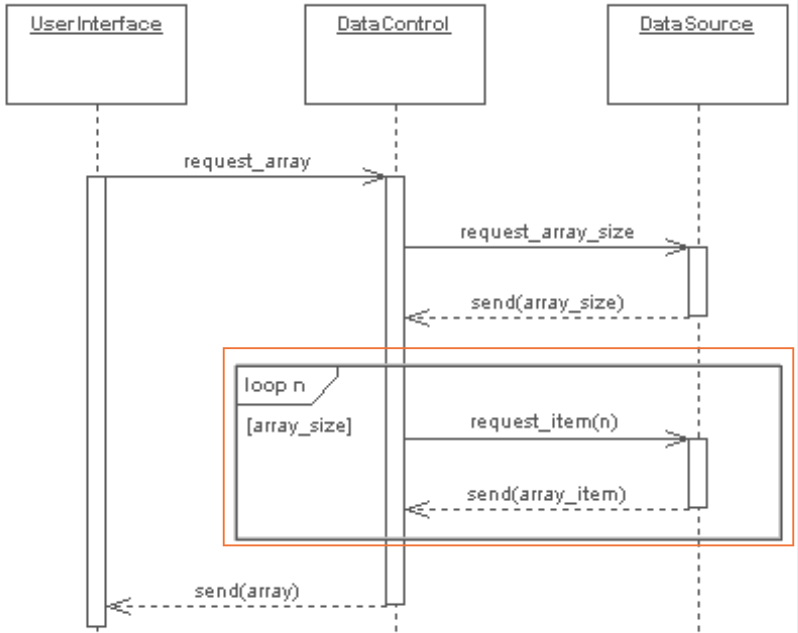
\includegraphics[width=0.6\linewidth]{res/teoria/SequenceDiagram.png}
    \caption{Sequence Diagram con fragment}
\end{figure}
\subsection{Activity diagram}
Un \textbf{activity diagram} è un diagramma di flusso che rappresenta un'operazione eseguita sul sistema, con decisioni, I/O, fork/join, timeout/segnali, concorrenza. Possiamo raggruppare alcune attività \textit{related}. 
Alcuni esempi di activity diagrams strani:
\begin{itemize}
    \item \textbf{State machine diagram}, che dà indicazioni a livello hardware
    \item \textbf{Choice and Junction pseudo state}
    \item \textbf{Compound state} tramite il quale possiamo separare alcune parti del diagramma e "includerle"
    \item \textbf{History state and concurrent regions}, con il primo indichiamo un salvataggio dello stato, col secondo due frazioni di diagramma che si svolgono contemporaneamente
\end{itemize}
\begin{figure}[H]
    \centering
    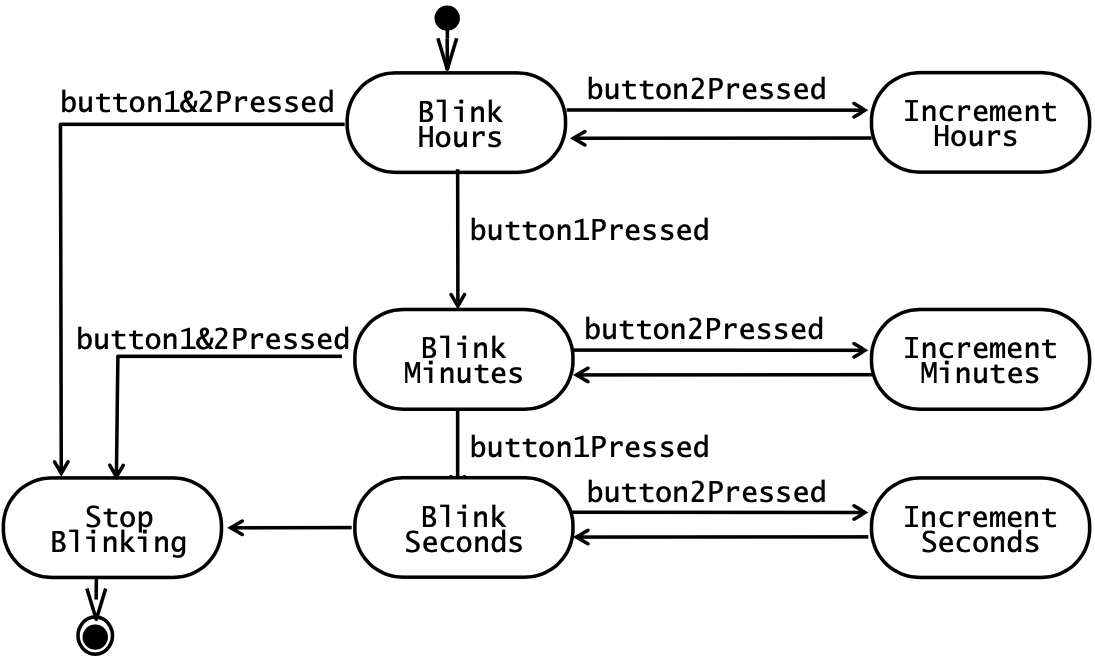
\includegraphics[width=0.6\linewidth]{res/teoria/StateMachine.png}
    \caption{State machine diagram}
\end{figure}
\subsection{Robustness diagram}
Il \textbf{robustness diagram} è un UML semplificato che ha lo scopo di raffinare gli use case, verificandone correttezza, completezza e requisiti.
Presenta tre \textbf{object nodes:}
\begin{itemize}
    \item \textbf{Boundary}, che permette la comunicazione tra attori e sistema
    \item \textbf{Control}, intermediario tra boundary ed entity, implementa la logica che gestisce i vari elementi e le loro interazioni
    \item \textbf{Entity}, rappresenta un'unità informativa del sistema
\end{itemize}
\begin{figure}[H]
    \centering
    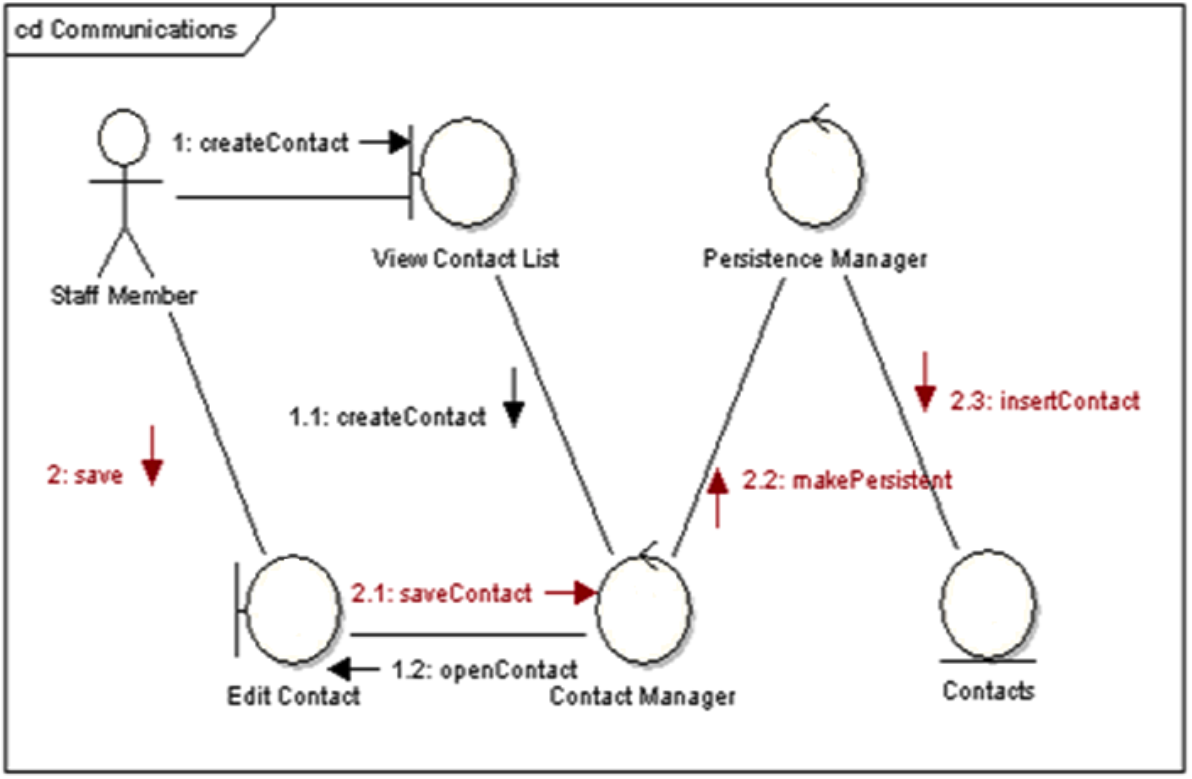
\includegraphics[width=0.4\linewidth]{res/teoria/Robustness.png}
    \caption{Robustness communication diagram}
\end{figure}
\section{T6 - Feasability and requirements elicitation}
Per ottenere le informazioni necessarie, dobbiamo identificare le fonti, acquisire le informazioni, analizzarle e verificarle. Infine, vanno sintetizzate. I vari stakeholder \textit{aka le persone interessate} possono essere così categorizzati con i loro interessi;
\begin{itemize}
    \item \textbf{Stakeholder}, interessato nel progetto
    \item \textbf{Developer}, alta produttività, mancanza di errori, minore sforzo possibile
    \item \textbf{Marketing sales}, soddisfazione del cliente e vendite
    \item \textbf{Project management}, budget, scadenze
    \item \textbf{Investor}, velocizzazione del processo
    \item \textbf{Customer and user}, usabilità e workflow
\end{itemize}
\subsection{Tecniche di elicitation}
\textit{(elicitation = tirare fuori le informazioni)}
\subsubsection{Document analysis}
Bisogna preparare i documenti che possono essere adatti e rilevanti, studiarli, annotare informazioni ed elencare le domande al riguardo. Infine, assieme agli stakeholder, verificare le note, organizzare i requirement e rispondere alle suddette domande. Questa tecnica può essere sfruttata quando non c'è presenza degli stakeholder, o per il cross-checking.
\subsubsection{Observation of the work environment}
L'obiettivo è determinare \textbf{chi, cosa, dove, quando, perché e come.} Bisogna ottenere il permesso dai supervisori, informare gli osservati, prendere appunti, evitare di disturbare ma al tempo stesso non dare nulla per scontato. I dati ottenuti sono molto affidabili.
\subsubsection{Questionario}
Serve determinare i fatti e le opinioni necessarie, in secundis, da chi reperirli. Determinare quindi le domande, aperte o chiuse, da fare. Può essere conveniente "testare" il questionario su un gruppo piccolo, per poi metterlo a posto e presentarlo a tutti. Questa tecnica restituisce molti dati, è facile da attuare ed affidabile. Non c'è però interazione, e si rischiano risposte incomplete. 
\subsubsection{Interviste}
Bisogna, prima di tutto, decidere chi intervistare. In seguito, preparare le domande e porle all'intervistato, con un linguaggio chiaro. Conviene prendere appunti e memo. Questo è un metodo ottimo perché permette di verificare i fatti, coinvolgendo gli end user. Non è però adatto a comprendere i domain requirements.
\subsubsection{Scenarios and use cases}
Essi sono esempi IRL di come il sistema verrà usato, basati su situazioni reali su cui gli stakeholder hanno senz'altro qualcosa da dire. Gli \textbf{scenari} sono semplicemente forme strutturare di user stories. Per gli use cases usiamo UML. Queste tecniche sono semplici ed utili, anche per sistemi complessi. È però difficile capire quando fermarsi, e soprattutto non sono utili a capire i \textbf{non-functional requirements.}
\subsection{Attività di supporto all'elicitation}
\subsubsection{Brainstorming}
Composto di due fasi, la prima di \textbf{storm} in cui si generano le idee, la seconda \textbf{calm} in cui vengono filtrate. Necessari due ruoli chiave: uno \textbf{scribe} ed un \textbf{moderatore}.
Nel filtraggio delle idee è fondamentale: unire idee simili, applicare i criteri di accettabilità, votare con una soglia o votare con dei \textit{campaign speeches.}
\subsubsection{Focus group}
Concetto simile al brainstorming ma più strutturato, esplora pro e contro di determinate opzioni. Fondamentale un moderatore.
\subsubsection{Prototypes}
Si mostra l'esecuzione di una task, si identificano le alternative, si cerca di estrapolare i possibili problemi. 
\section{T7 - Use Cases}
Gli \textbf{use case} sono scenari che sfruttano diagrammi UML, descrivono le task del sistema e l'interazione con gli attori. Non sono mappati one-to-one coi requirements, ma ogni requirement deve essere coperto da almeno uno use case. Gli use case sono quindi composti da use case diagrams, descrizioni testuali, ed interaction diagrams (opzionali).
Per identificare gli actor bisogna definire prima i boundary, poi gli utenti, l'hardware, i ruoli. Per identificare gli use case bisogna prima identificare il dominio. Vanno poi annotati come verbi rappresentanti le azioni. Per l'identificazione degli scenari, bisogna comprendere la situazione iniziale e il flusso di eventi. È utile capire cosa può andare male, e tutti i flussi alternativi. Infine, consideriamo la situazione finale. Uno use case deve avere un singolo attore iniziante, pochi step, non deve includere scelte implementative, può includere UML. Bisogna poi dare una priorità ai vari use case, in base all'impatto, la difficoltà, la necessità. 
\subsection{Componenti principali}
Uno use case deve definire lo stato iniziale e le precondizioni. Deve definire l'ordine degli eventi, le alternative, le situazioni eccezionali, e i risultati. Deve inoltre menzionare gli attori coinvolti, i diagrammi related, i problemi di design. Alcune guidelines:
\begin{itemize}
    \item Non pensare al lato implementativo
    \item Essere narrativi
    \item Elencare gli scenari funzionanti
    \item Elencare tutti i possibili use case
    \item Utilizzare un formato standard
    \item Utilizzare i verbi appropriati
    \item Documentare le eccezionali
    \item Non rappresentare singoli step come use cases
\end{itemize}
\begin{figure}[H]
    \centering
    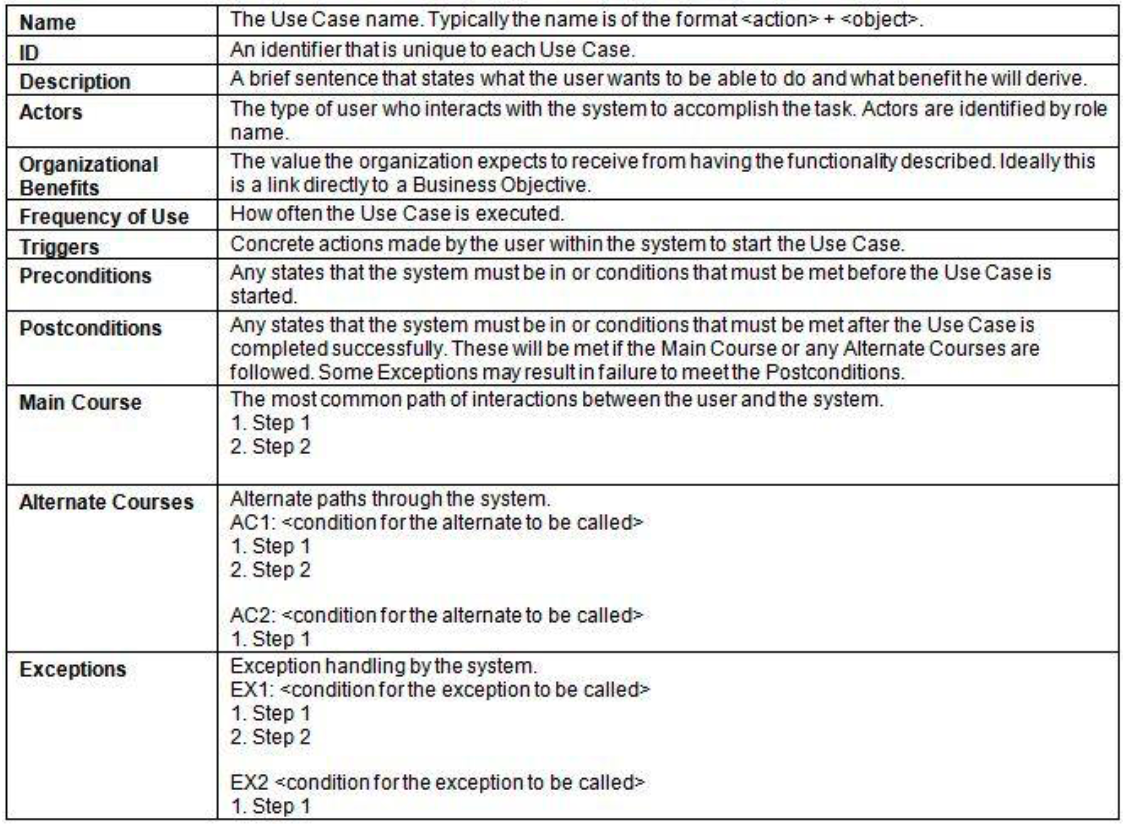
\includegraphics[width=0.8\linewidth]{res/teoria/UseCaseTemplate.png}
    \caption{Use case template}
\end{figure}

\section{T8 - Requirements Analysis}
L'analisi dei requirements raffina e struttura i requisiti in modo da renderli più chiari, precisi e formali. Esso definisce l'\textit{analysis model}, che raffina la descrizione informale dei requirement e la converte in diagrammi di flusso. Il suddetto non è un modello di design, ed è indipendente dalla piattaforma. Descrive le funzionalità che il sistema deve realizzare. 
\subsection{Analysis Classes}
Il concetto è quello di astrarre le entità del problema. Bisogna gestire i functional requirements (i non-functional sono gestiti nel \textbf{design architetturale}). Incorpora un set minimale di \textbf{responsabilità}. Questa analisi è rappresentata con digrammi di classe.
\subsection{Classes discovering techniques}
Esistono diverse tecniche atte a scovare le classi coinvolte. Procediamo ad elencarne le più importanti.
\subsubsection{Noun verb analysis}
Questa analisi sfrutta i documenti contenenti le specifiche di progetto, cercandovi nomi e verbi. Pare ovvio che la completezza dei documenti è fondamentale. La qualità dipende anche dallo stile di scrittura dei requisiti. 
\subsubsection{Use case driven approach}
Questo approccio sfrutta gli scenari di use case, e dipende quindi dalla correttezza dei suddetti. 
\subsubsection{Common Class Patterns}
Quest'analisi si basa sulla teoria della \textbf{classificazione generica degli oggetti}. Essa fornisce delle linee guida, ma non un processo sistematico atto ad ottenere le classi. Porta diversi rischi, tra cui quello di possibili interpretazioni errate dei nomi. 
\begin{figure}[H]
    \centering
    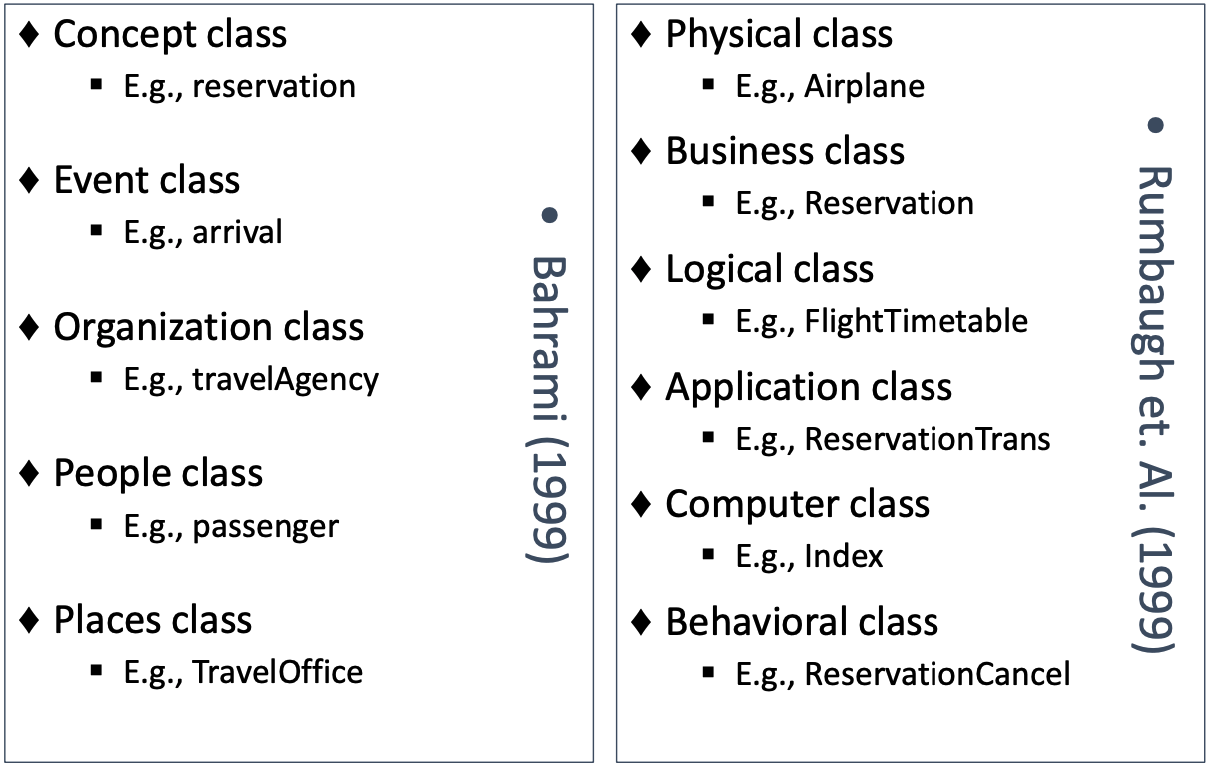
\includegraphics[width=\linewidth]{res/teoria/CommonClassPatterns.png}
    \caption{Common Class Patterns}
\end{figure}
\subsubsection{CRC Cards}
Le \textbf{CRC Cards} sono utilizzate in specifiche sessioni di brainstorming. Generalmente si parte dagli use cases, e si creano delle card con:
\begin{itemize}
    \item Class name
    \item Responsibilities
    \item Collaborators
\end{itemize}
Non viene fornito un metodo sistematico, e per questo le CRC cards sono piuttosto un mezzo di validazione dei requirements. 
\begin{figure}[H]
    \centering
    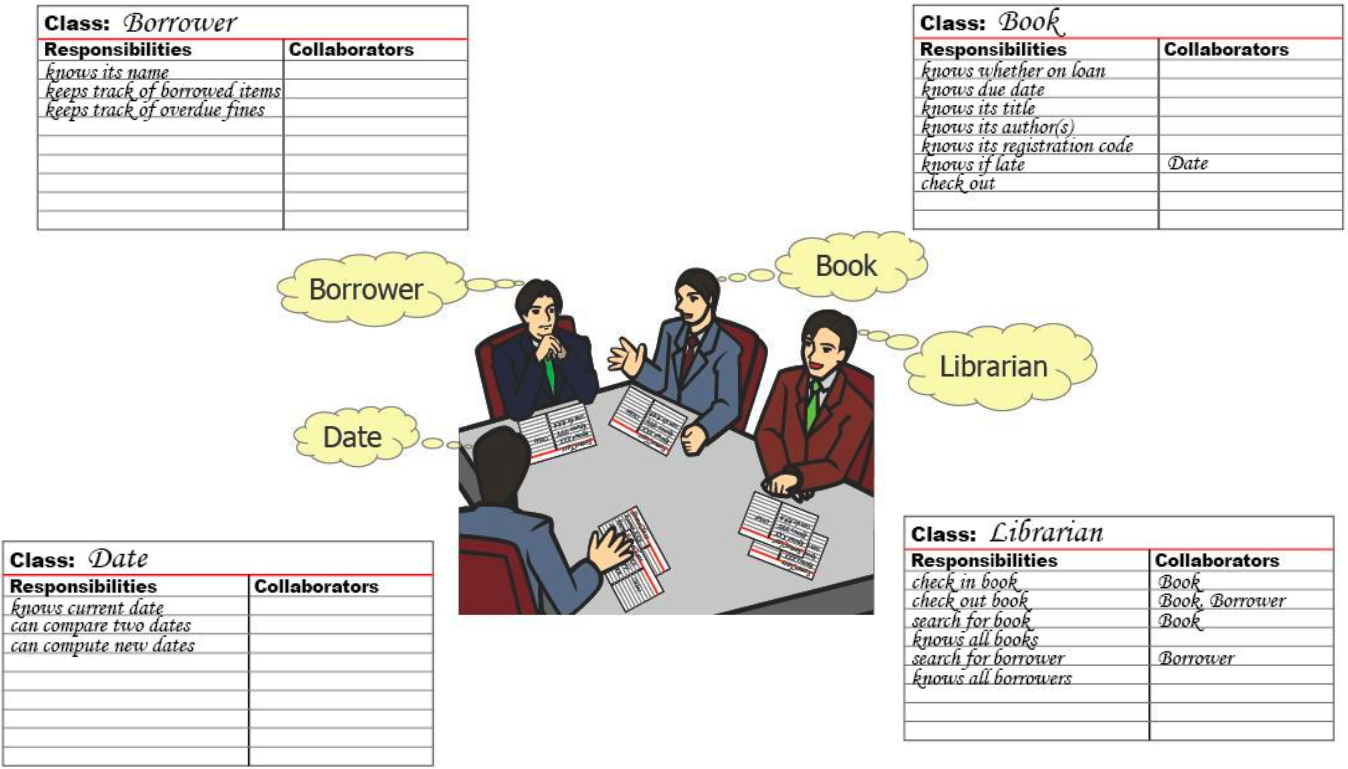
\includegraphics[width=\linewidth]{res/teoria/CRCCards.png}
    \caption{CRC Cards}
\end{figure}
Gli achievement di questo metodo sono:
\begin{itemize}
    \item Verificare la correttezza dello use case
    \item Verificare la correttezza delle associazioni
    \item Verificare la correttezza delle generalizzazioni
    \item Trovare le classi omesse
    \item Scovare opportunità di refactor
\end{itemize}
\subsection{Mixed approach}
Come sempre, la via di mezzo è quella vincente:
\begin{enumerate}
    \item Le classi iniziali provengono dalla conoscenza del dominio
    \item Si sfrutta, come guida, il common class pattern
    \item Per aggiungere altre classi, noun verb analysis
    \item Per verificare il lavoro, Use Case approach
    \item Per il brainstorming, CRC
\end{enumerate}
\section{T9 - Requirements Validation and Management}
\subsection{Validation}
La validazione consiste nel verificare la correttezza dei requirement, con due obiettivi principali: \textbf{completezza} e \textbf{costi}. Inoltre:
\begin{itemize}
    \item \textbf{Consistency}: assenza di conflitti
    \item \textbf{Realism}: possono essere effettivamente implementati?
    \item \textbf{Verifiability}: possono essere verificati?
\end{itemize}
La review dei requirement dovrebbe essere svolta continuamente durante la loro stesura. Essa deve essere svolta sia dal progettista che dal cliente. Alcuni issue da verificare sono:
\begin{itemize}
    \item Verifiability: il requirement è testabile?
    \item Comprehensibility: il requirement è stato compreso correttamente?
    \item Traceability: l'origine del requirement è chiara?
    \item Adaptability: i requirement possono essere cambiati senza impatti sul resto?
\end{itemize}
\begin{figure}[H]
    \centering
    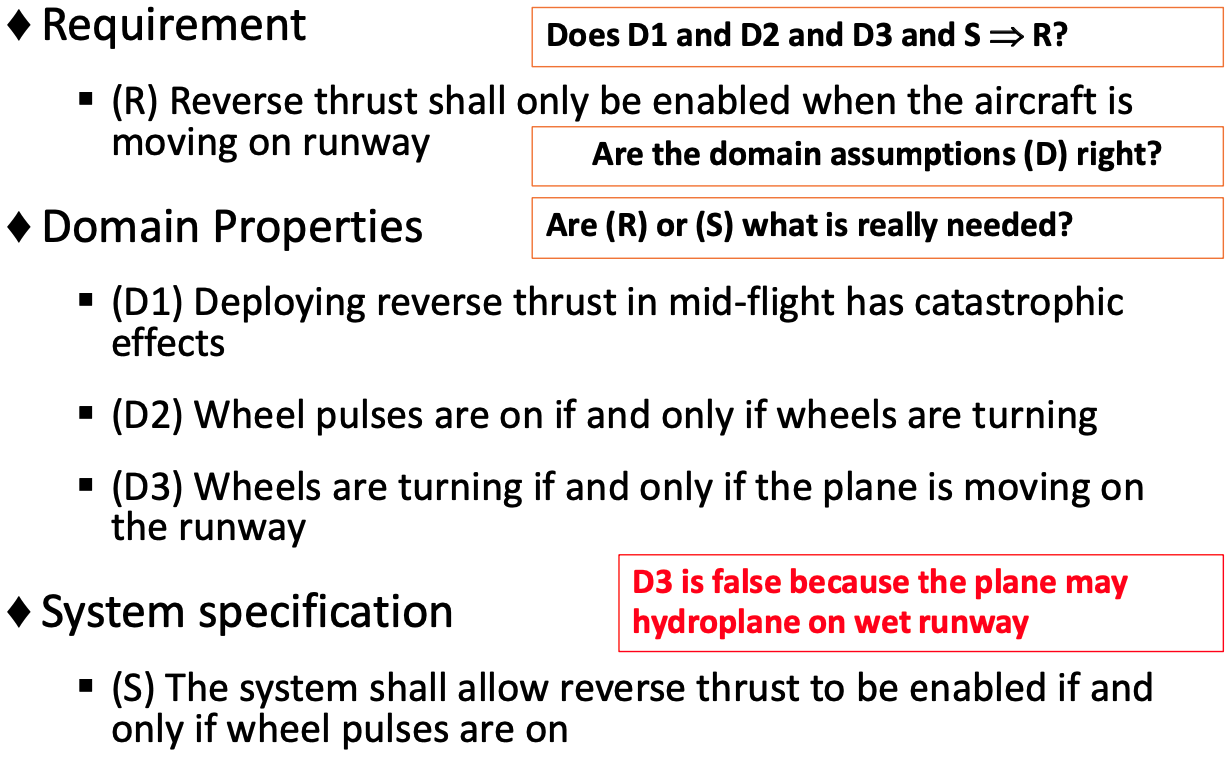
\includegraphics[width=\linewidth]{res/teoria/RequirementReview.png}
    \caption{Esempio di requirement review}
\end{figure}
\subsection{Requirements management}
Si verificano errori, conflitti ed inconsistenze. Vanno tenuti in conto i lati tecnici, la schedule, i costi, seguendo le priorità del cliente. 
Va quindi stimato il costo del progetto, controllata la requirements \gls{volatility}, negoziati i cambiamenti, ri-stimati i costi. L'interesse è soddisfare il cliente, rimanendo nel budget. 
Le necessità del requirement management sono:
\begin{itemize}
    \item Identificazione dei requirement
    \item Un processo di modifica
    \item Policy di tracciabilità
    \item Supporto del \gls{case}
\end{itemize}
\subsubsection{CASE tool support}
I requirement devono essere salvati in una zona sicura. Il change management deve essere un processo di workflow con passaggi definiti, e, se possibile, automatizzati. \textit{Immaginatelo come un Github Actions, ma nel 95.} Deve inoltre esserci un'automatizzazione dei link tra requirement, rinforzando la tracciabilità.
\subsubsection{Identificazione dei requirement}
I requirement devono essere identificati univocamente. Potremmo quindi numerare capitoli/sezioni, ma \textit{come fa un po' schifo come approccio.} Per questo, sfruttiamo una numerazione dinamica, identificante i record nel DB. Potremmo sfruttare un'identificazione simbolica, con, ad esempio, sigle. \textit{Se usi degli issue tracker, è lo stesso concetto dei codici tra quadre.}
\subsubsection{Stati dei requirement}
I requirement possono avere degli stati (\textit{Anche qui, aver usato issue tracker può chiarire il concetto}):
\begin{itemize}
    \item Proposed
    \item Approved
    \item Rejected
    \item Implemented
    \item Verified 
    \item Deleted
\end{itemize}
\subsubsection{Change management}
È una buona idea implementare un version control dei requirement, per poter tracciare i cambiamenti. Prima di modificare un requirement, è importante analizzare il problema, i costi, e le specifiche. 
\begin{figure}[H]
    \centering
    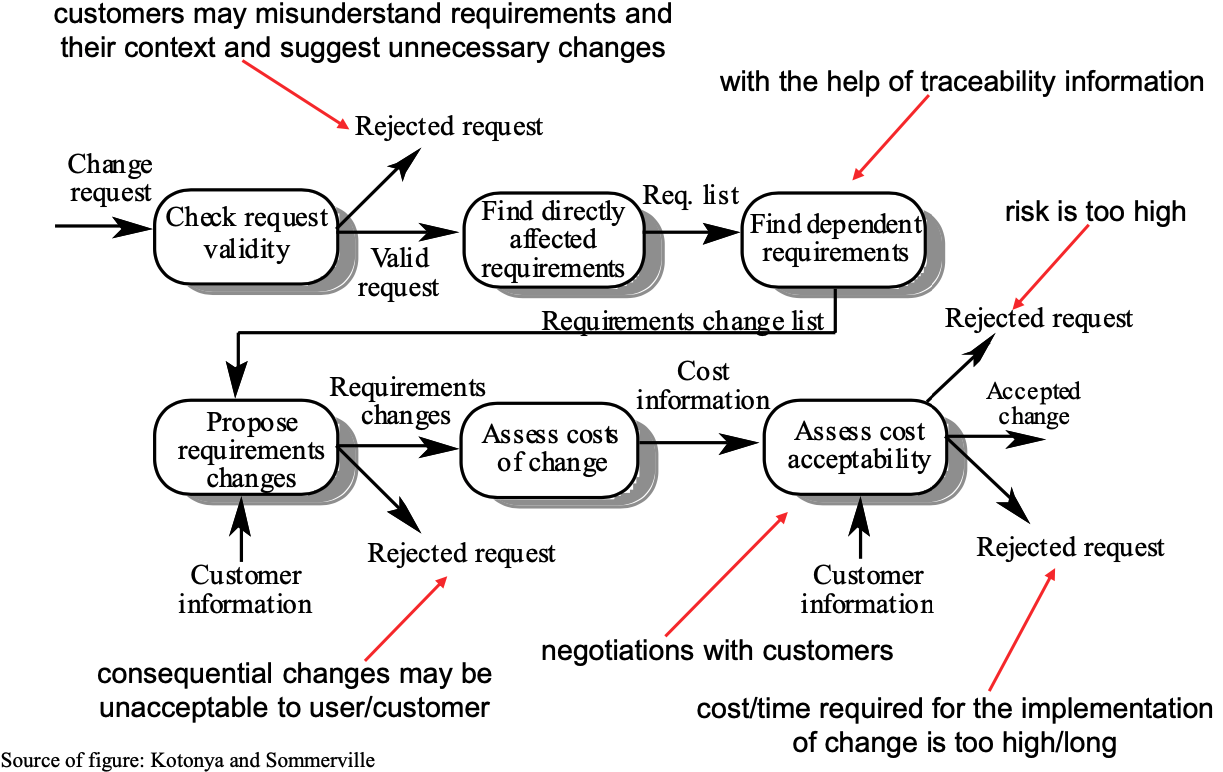
\includegraphics[width=\linewidth]{res/teoria/ChangeManagement.png}
    \caption{Change management diagram}
\end{figure}
\subsection{Traceability}
Lo sviluppo produce relazioni: predecessore-successore, master-subordinate. È fondamentale identificare queste relazioni ed il loro grado, allo scopo di tenere traccia dei \textit{path} nelle gerarchie. Alcuni esempi di traceability:
\begin{itemize}
    \item User needs $\rightarrow$ Product features
    \item Requirements $\rightarrow$ Implementation
    \item Use case $\rightarrow$ Test case
\end{itemize}
Distinguiamo tra vari tipi di traceability:
\begin{itemize}
    \item \textbf{Source}: la persona o il documento che hanno richiesto il requirement
    \item \textbf{Rationale}: fonte delle informazioni che descrivono le motivazioni del requirement
    \item \textbf{Requirements}: alcuni requirement sono collegati ad altri, da cui dipendono
    \item \textbf{Architecture}: collega i requirement ai sottosistemi in cui sono implementati
    \item \textbf{Design}: collega i requirement con specifici software/hardware necessari all'implementazione
    \item \textbf{Interface}: collega l'interfaccia di sistemi esterni che hanno reso necessario il requirement
    \item \textbf{Feature}: collega il requirement ai suoi componenti
    \item \textbf{Tests}: collega il requirement ai test cases che lo verificano
    \item \textbf{Code}: generalmente non stabilito direttamente, ma può essere implicato
\end{itemize}
Nella tracciabilità, si può incappare in diversi issue:
\begin{itemize}
    \item Gli stakeholder richiedono informazioni diverse
    \item Elevata quantità di informazioni richieste
    \item Problemi nel management manuale
    \item Necessità di tool specializzati
    \item Problemi di integrazione
\end{itemize}
\subsubsection{Traceability Planning}
Elementi fondamentali al planning sono:
\begin{itemize}
    \item Tipi di stakeholder
    \item Informazioni richieste
    \item Dove e da chi raccogliere informazioni
    \item Dove e come mantenere le informazioni 
    \item Dove e come cercare le informazioni
\end{itemize}
Abbiamo inoltre dei \glspl{constraint} al planning: 
\begin{itemize}
    \item \textbf{Numero di requirements}: maggiore è il numero di requirement, più sono necesarie delle policy formali di tracciabilità
    \item \textbf{Expected system lifetime}: in caso di lunghe lifetime, sono necessarie policy di tracciabilità più comprensive
    \item \textbf{Livello di maturità dell'organizzazione}: in organizzazioni con un'elevata maturità di processo vengono usate policy più dettagliate
    \item \textbf{Dimensioni di progetto e team}: maggiori le dimensioni, maggiore la formalità richiesta
    \item \textbf{Tipo di sistema}: sistemi critici come quelli real-time, o richiedenti sicurezza, hanno bisogno di policy di tracciabilità migliori
    \item \textbf{\Gls{constraint} addizionali del cliente}: il cliente può necessitare \gls{constraint} vari, ad esempio standard militari
\end{itemize}
\textit{I più svegli di voi si chiederanno perché passo dalla lezione 9 alla 12. La risposta è semplice, la 10 e la 11 sono dei doppioni di 8 e 9.}
\section{T12 - Object Constraint Language}
I diagrammi UML spesso non sono abbastanza raffinati per descrivere tutti i constraint sulle relazioni tra entità. Per questo, spesso, essi sono espressi tramite il linguaggio naturale, coi soliti problemi di ambiguità, o con un linguaggio formale, non comprensibile ai più. 
L'\textbf{Object Constraint Language} fa parte delle specifiche UML, ed è un linguaggio formale con sintassi e semantiche definite. Permette di descrivere espressioni e constraint tramite modelli object-oriented. È semplice da leggere e fu sviluppato da niente meno che \textbf{IBM}. Può essere utilizzato in vari modi:
\begin{itemize}
    \item Come query language
    \item Per specificare constraint su classi e tipi
    \item Per specificare constraint su operazioni
    \item Per specificare target su messaggi e azioni
    \item Per definire espressioni utili alla navigazione tra modelli UML
    \item Per testare requirement e specifiche
\end{itemize}
Definiamo tra 3 data types: quelli basic, quelli user-defined e le collection. È possibile eseguire operazioni booleane, operazioni reali/intere. Sono disponibili vari tipi di collection, tra cui nominiamo i set, gli ordered set, le bag \textit{(no, non quelle bag)}, in cui gli elementi possono essere ripetuti, e le sequenze, che sono bag ordinate.
Le collection hanno delle operazioni (le classiche operazioni da collection), come \code{size}, \code{isEmpty}, \code{notEmpty}, \code{sum}, \code{count}, \code{includes}, \code{includesAll}.
\subsection{Model types}
I \textbf{model types} sono classi, subclasses, classi di associazione, interfacce, enumerazioni. Hanno proprietà, come attributi, metodi, navigazioni (derivate dalle associazioni), enumerazioni. Possono essere inoltre \textit{referenziate} in espressioni OCL.
\subsection{Operazioni, espressioni, constraints}
Abbiamo alcune operazioni di base, come \code{oclIsTypeOf(type: OclType)}, o \code{oclIsKindOf}. Ogni espressione, contenente operazioni query, restituisce un risultato. Il tipo dell'espressione è il tipo del risultato. Un constraint è semplicemente un'espressione booleana. 
I constraint sono quindi restrizioni su uno o più valori di un modello/sistema object-oriented. Sono dichiarativi, non hanno \textit{side effects}, ed hanno sintesi formale e semantiche. Perché si usano?
\begin{itemize}
    \item Migliore documentazione
    \item Più precisione
    \item Comunicazione senza ambiguità
\end{itemize}
Abbiamo svariati tipi di constraint:
\begin{itemize}
    \item \textbf{Invariant}: deve essere vero quando l'istanza è a riposo
    \item \textbf{Pre-condition}: deve essere vero quando un'operazione è invocata
    \item \textbf{Post-condition}: deve essere vero dopo il completamento di un'operazione
    \item \textbf{Guard}: deve essere vero prima che una transizione possa accadere, quindi è una specie di pre-condition
\end{itemize}
La sintassi è semplice: \code{[termine del constraint][nome del constraint]:[espressione booleana]}. I termini per i constraint suddetti sono \code{inv}, \code{pre}, \code{post}, \code{pre/post…implies oclInState}.




\printglossary

\end{document}